\chapter*{script Hello World dan {Variable Explorer}
\begin{enumerate}
	\item menuliskan script hello world di spyder
	\begin{figure} [h]
	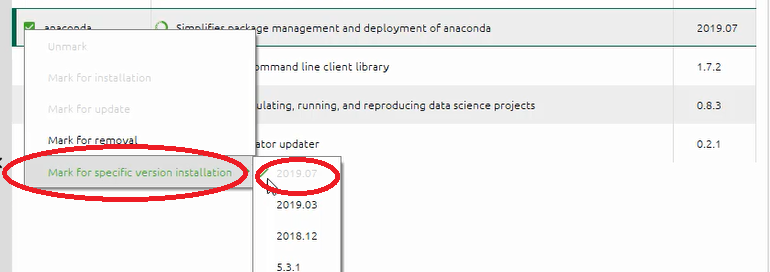
\includegraphics[width=5cm]{update/4.png}
	\centering
	\end{figure}	
\begin{enumerate}
	\item menuliskan seperti yang ada di gambar disini x merupakan variable dan puja merupakan value 
	\begin{figure} [h]
	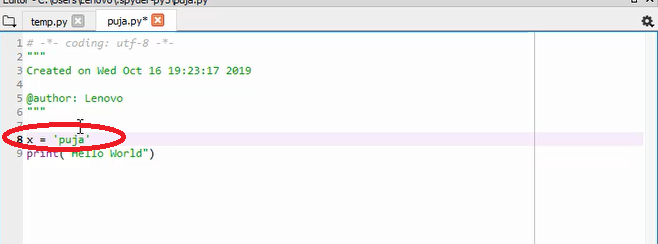
\includegraphics[width=5cm]{variable/1.png}
	\centering
	\end{figure}	
	\item Ikuti seperti digambar maksudnya adalah hello + value dari variable yang sudah dibuat sebelumnya 
	\begin{figure} [h]
	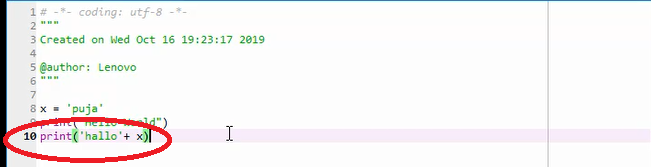
\includegraphics[width=5cm]{variable/2.png}
	\centering
	\end{figure}
	\item dan akan jadi seperti yang ada digambar 
	\begin{figure} [h]
	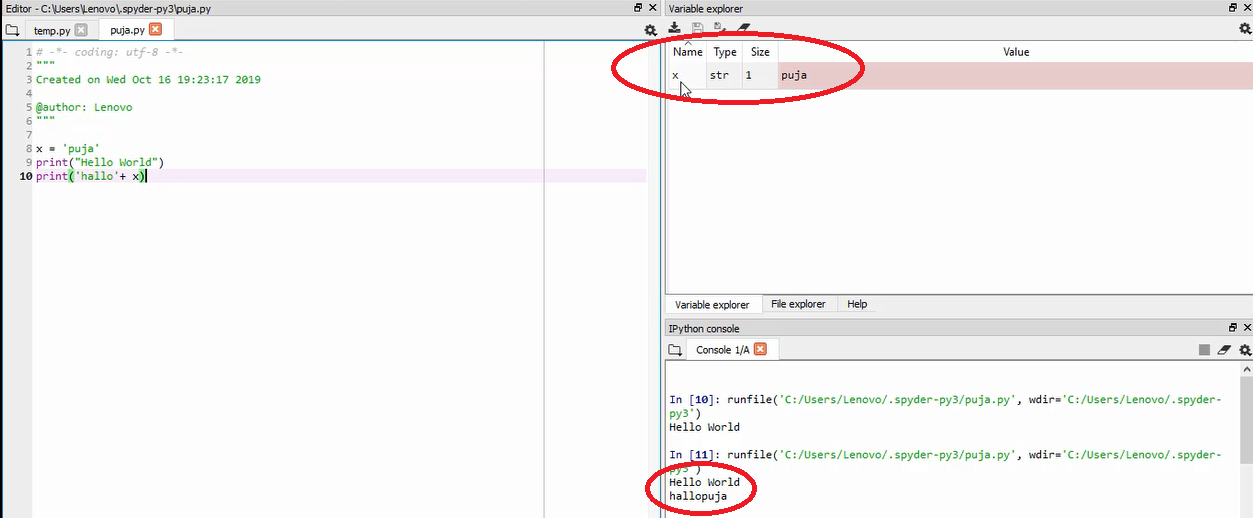
\includegraphics[width=5cm]{variable/3.png}
	\centering
	\end{figure}	
	\item mengupdate Anaconda sama hal nya seperti mengupdate spyder hanya berbeda saat mecari, ketikan "Anaconda" dan ikuti seperti digambar
	\begin{figure} [h]
	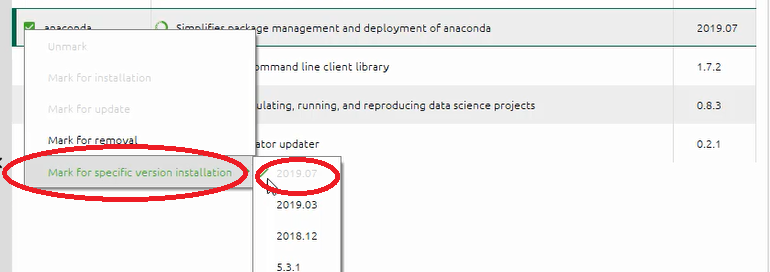
\includegraphics[width=5cm]{update/4.png}
	\centering
	\end{figure}		
\end{enumerate}
